%!TEX root = art-in-machine-learning.tex

\section{Image Data}\label{sec:images}%
Applying a simple neural network on image data directly can work, but the number
of parameters gets extraordinary large. One would take one neuron per pixel and
channel. This means for $\SI{500}{\pixel} \times \SI{500}{\pixel}$ RGB images
one would get \num{750000} input signals. To approach this problem, so called
\glspl{CNN} were introduced. Instead of learning the full connection between
the input layer and the first hidden layer, those networks make use of
convolution layers. Convolution layers learn a convolution; this means they
learn the weights of an image filter. An additional advantage is that
\glspl{CNN} make use of spacial relationships of the pixels instead of
flattening the image to a stream of single numbers.

An excellent introduction into \glspl{CNN} is given by~\cite{Nielsen2015}.


\subsection{Google DeepDream}\label{subsec:google-deepdream}%
The gradient descent algorithm which optimizes most of the parameters in neural
networks is well-understood. However, the effect it has on the recognition
system is difficult to estimate. \cite{inceptionism2015} proposes a technique
to analyze the weights learned by such a network. A similar idea was applied
by~\cite{vondrick2013hoggles}.

For example, consider a neural network which was trained to recognize various
images like bananas. This technique turns the network upside down and starts
with random noise. To analyze what the network considers bananas to look like,
the random noise image is gradually tweaked so that it generates the output
\enquote{banana}. Additionally, the changes can be restricted in a way that the
statistics of the input image have to be similar to natural images. One example
of this is that neighboring pixels are correlated.
\goodbreak
Another technique is to amplify the output of layers. This was described
in~\cite{inceptionism2015}:\nobreak%
\begin{displayquote}
We ask the network: \enquote{Whatever you see there, I want more of it!} This
creates a feedback loop: if a cloud looks a little bit like a bird, the network
will make it look more like a bird. This in turn will make the network
recognize the bird even more strongly on the next pass and so forth, until a
highly detailed bird appears, seemingly out of nowhere.
\end{displayquote}

\begin{figure}[ht]
    \centering
    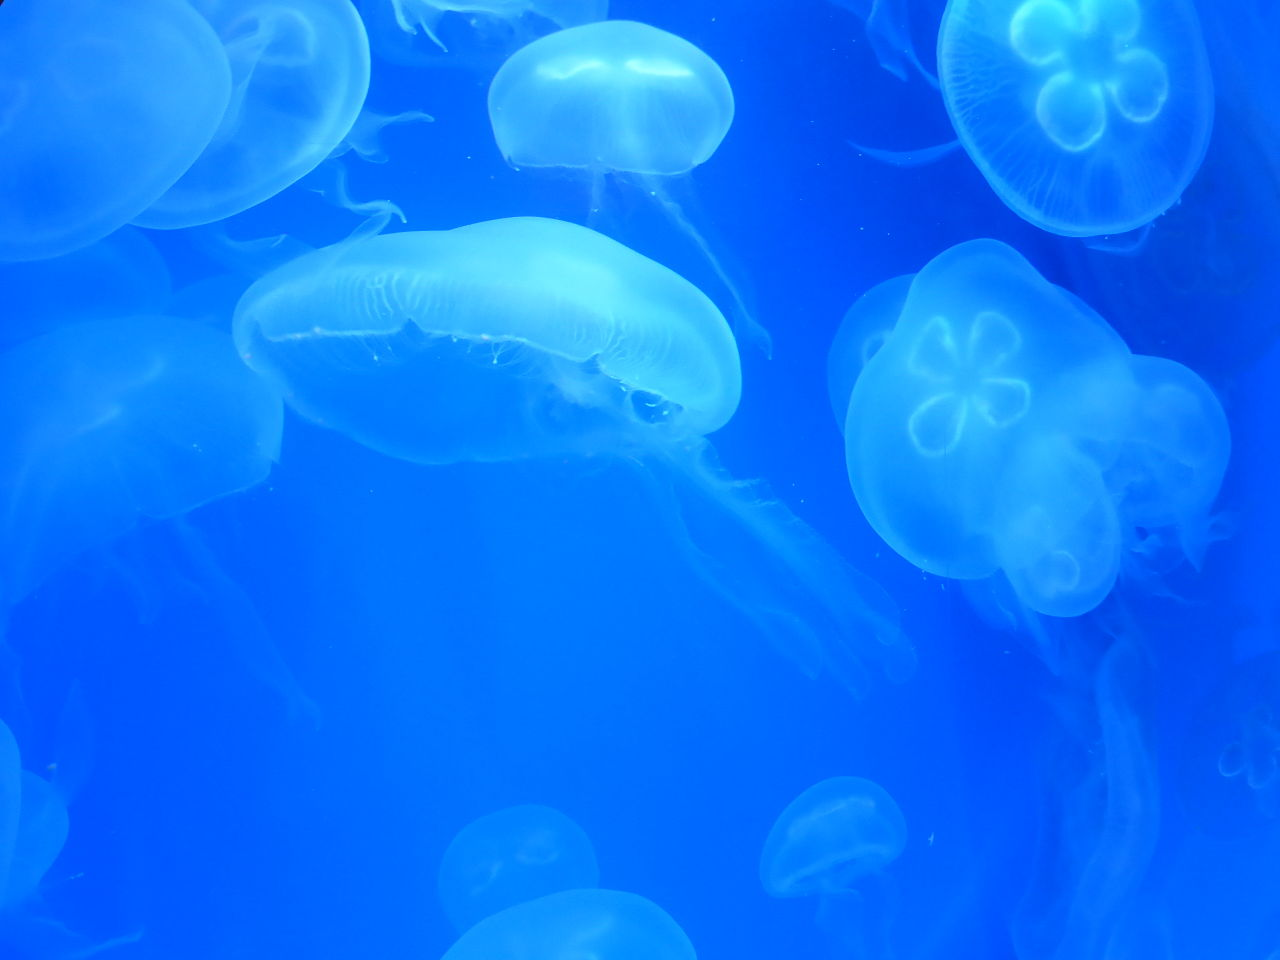
\includegraphics[width=0.45\textwidth]{figures/DeepDream/Aurelia-aurita-3/Aurelia-aurita-3.jpg}
    \caption{Aurelia aurita}
    \label{fig:Aurelia-aurita-3-original}
\end{figure}

\begin{figure}[ht]
    \centering
    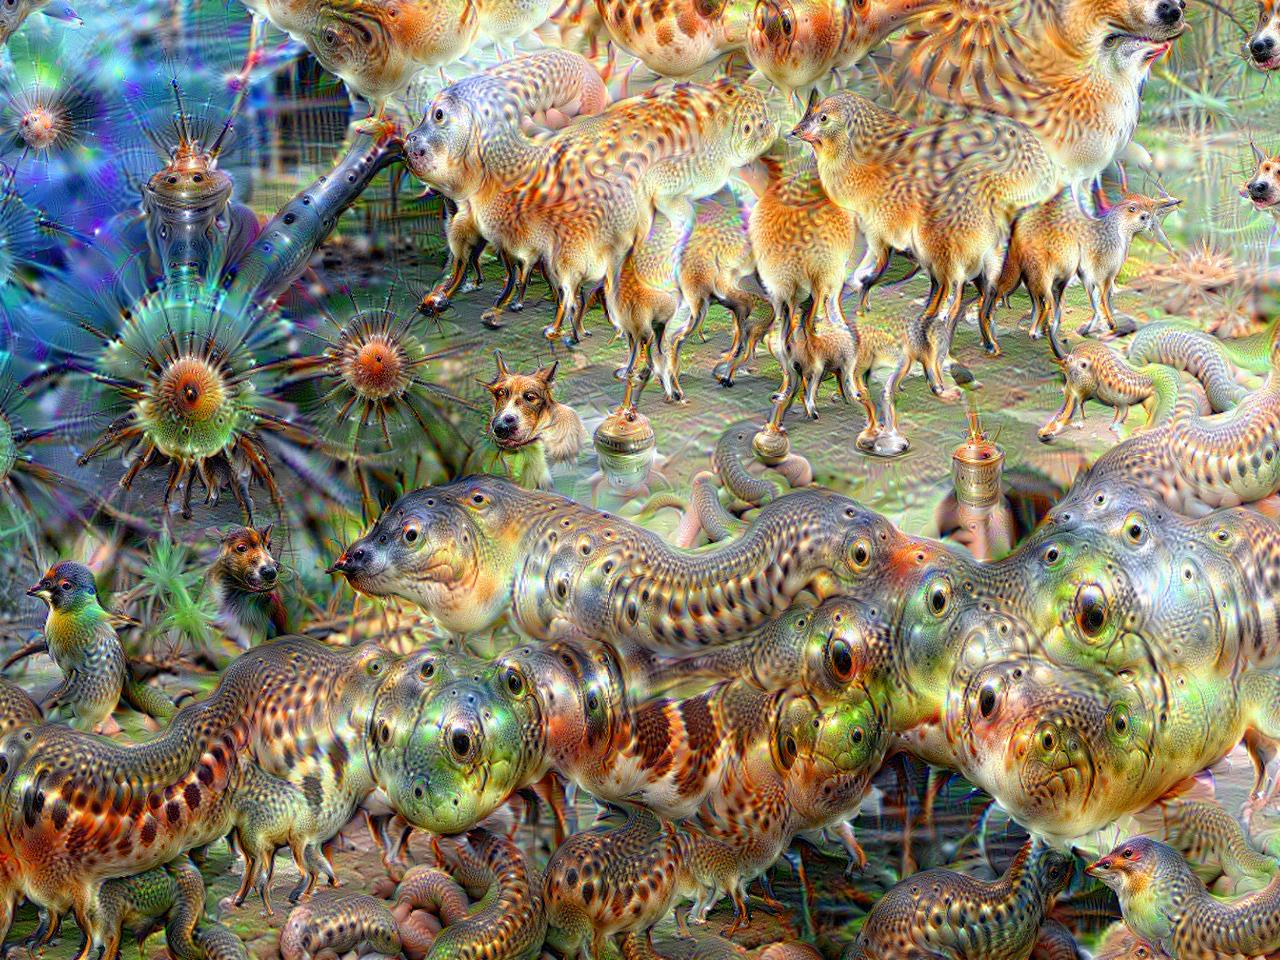
\includegraphics[width=0.45\textwidth]{figures/DeepDream/Aurelia-aurita-3/0099.jpg}
    \caption{DeepDream impression of Aurelia aurita}
    \label{fig:Aurelia-aurita-3-100}
\end{figure}

The name \enquote{Inceptionism} in the title of~\cite{inceptionism2015} comes
from the science-fiction movie \enquote{Inception}~(2010). One reason it might
be chosen is because neural networks are structured in layers. Recent
publications tend to have more and more layers~\cite{he2015deep}. The used
jargon is to say they get \enquote{deeper}. As this technique as published by
Google engineers, the technique is called \textit{Google DeepDream}.

It has become famous in the internet~\cite{RedditDeepDream}. Usually, the
images are generated in iterations and in each iteration it is zoomed into the
image.\\
Images and videos published by the Google engineers can be seen
at~\cite{googlePhotos2015}. \Cref{fig:Aurelia-aurita-3-original} shows the
original image from which \cref{fig:Aurelia-aurita-3-100} was created with the
deep dream algorithm.


% \subsection{Caption generation}
% Generating captions for images can be seen as a creative task, too. Interesting
% captions don't only describe what one can obvioulsy see on the image, but also
% interpret the image to a certain degree.


\subsection{Artistic Style Imitation}
A key idea of neural networks is that they learn different representations of
the data in each layer. In the case of \glspl{CNN}, this can easily be
visualized as it was done in various papers~\cite{zeiler2014visualizing}.
Usually, one finds that the network learned to build edge detectors in the
first layer and more complex structures in the upper layers.

\begin{figure}
\centering
\subfigure[Original Image]{
  \label{fig:scottish-highland-cattle}
  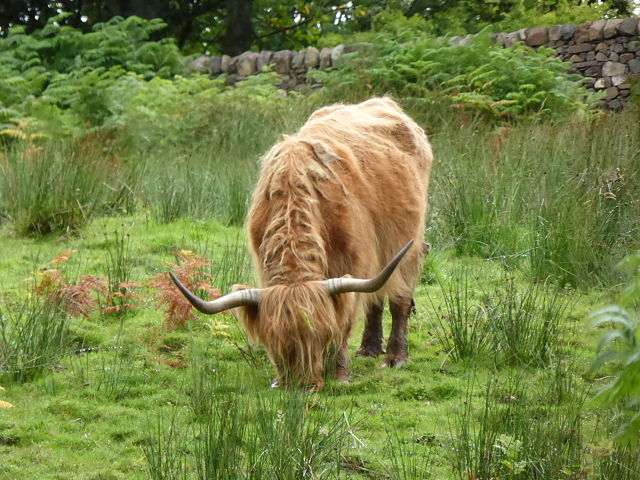
\includegraphics[width=0.45\linewidth, keepaspectratio]{figures/Artistic-Style/highland-cattle.jpg}
}%
\subfigure[Style image]{
  \label{fig:starry-night}
  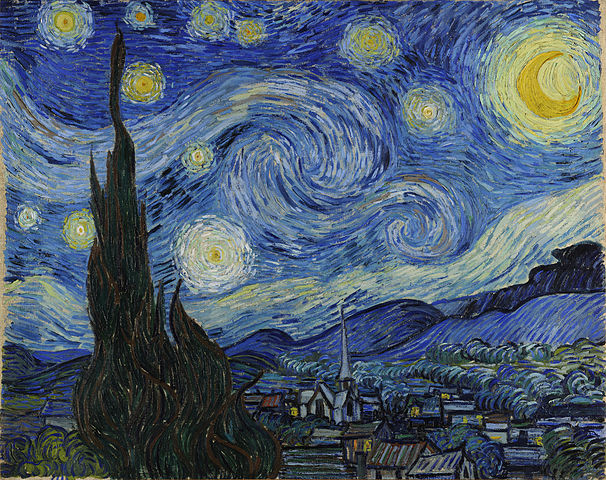
\includegraphics[width=0.45\linewidth, keepaspectratio]{figures/Artistic-Style/starry-night.jpg}
}

\subfigure[The artistic style of Van Gogh's \enquote{Starry Night} applied to the photograph of a Scottish Highland Cattle.]{
  \label{fig:highland-van-gogh}
  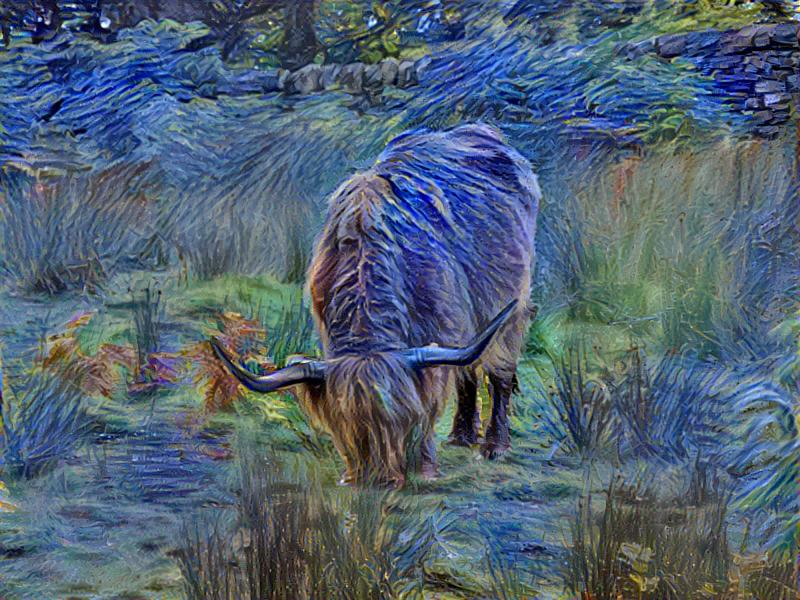
\includegraphics[width=0.93\linewidth, keepaspectratio]{figures/Artistic-Style/Scottish-highland-cattle-1-style.jpg}
}
\caption{The algorithm takes both, the original image and the style image  to produce the result.}
\label{fig:neural-style}
\end{figure}

Gatys, Ecker and Bethge showed in~\cite{gatys2015neural} that with a clever
choice of features it is possible to separate the general style of an image in
terms of local image appearance from the content of an image. They support
their claim by applying the style of different artists to an arbitrary image of
their choice.

This artistic style imitation can be seen itself as creative work. An example
is given by~\cref{fig:neural-style}. The code which created this example is
available under~\cite{Johnson2016}.

Something similar was done by~\cite{shih2014style}, where the style of a
portrait photograph was transferred to another photograph. A demo can be seen
on~\cite{Shih2014}.


\subsection{Drawing Robots}
Patrick Tresset and Fr\'{e}d\'{e}ric Fol Leymarie created a system called AIKON
(Automatic IKONic drawing) which can automatically generated sketches for
portraits~\cite{tresset2005generative}. AIKON takes a digital photograph,
detects faces on them and sketches them with a pen-plotter.

Tresset and Leymaire use $k$-means clustering~\cite{1017616} to segment regions
of the photograph with similar color which, in turn, will get a similar
shading.

Such a drawing robot could apply machine learning techniques known from
computer vision for detecting the human. It could apply self-learning
techniques to draw results most similar to the artists impression of the image.
However, the system described in~\cite{tresset2005generative} seems not to be a
machine learning computer program according to the definition by Tom
Mitchell~\cite{Mitchell97}.
